% Figure 5: Health Monitoring State Machine
\documentclass[tikz,border=5pt]{standalone}
\usepackage{tikz}
\usetikzlibrary{arrows.meta,positioning,automata}

\begin{document}
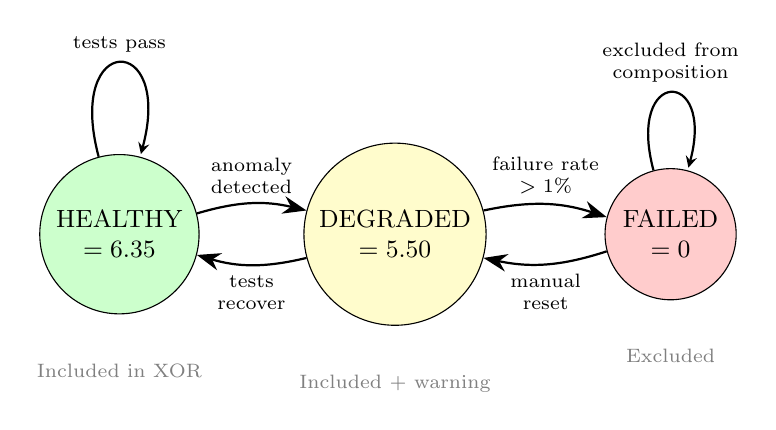
\begin{tikzpicture}[
  ->,>=stealth,
  node distance=3.5cm,
  every state/.style={draw, rounded corners, minimum size=1.5cm, align=center, font=\small},
  every edge/.style={draw, -{Stealth[length=3mm]}, thick},
  label/.style={font=\scriptsize, text=black, align=center},
]

% States
\node[state, fill=green!20] (healthy) {HEALTHY\\$\minentropy = 6.35$};
\node[state, fill=yellow!20, right of=healthy] (degraded) {DEGRADED\\$\minentropy = 5.50$};
\node[state, fill=red!20, right of=degraded] (failed) {FAILED\\$\minentropy = 0$};

% Transitions
\path (healthy) edge[bend left=15] node[above, label] {anomaly\\detected} (degraded);
\path (degraded) edge[bend left=15] node[below, label] {tests\\recover} (healthy);
\path (degraded) edge[bend left=15] node[above, label] {failure rate\\$> 1\%$} (failed);
\path (failed) edge[bend left=15] node[below, label] {manual\\reset} (degraded);

% Self-loops
\path (healthy) edge[loop above] node[label] {tests pass} (healthy);
\path (failed) edge[loop above] node[label] {excluded from\\composition} (failed);

% Annotations
\node[font=\scriptsize, text=gray, below=0.5cm of healthy] {Included in XOR};
\node[font=\scriptsize, text=gray, below=0.5cm of degraded] {Included + warning};
\node[font=\scriptsize, text=gray, below=0.5cm of failed] {Excluded};

\end{tikzpicture}
\end{document}
